%%%%%%%%%%%%%%%%%%%%%%%%%%%%%%%%%%%%%%%%%%%%%%%%%%%%%%%%%%%%%%%%%%%%%%%%%%%%%%%%
%2345678901234567890123456789012345678901234567890123456789012345678901234567890
%        1         2         3         4         5         6         7         8

\documentclass[letterpaper, 10 pt, conference]{ieeeconf}  % Comment this line out
                                                          % if you need a4paper
%\documentclass[a4paper, 10pt, conference]{ieeeconf}      % Use this line for a4
                                                          % paper

\IEEEoverridecommandlockouts                              % This command is only
                                                          % needed if you want to
                                                          % use the \thanks command
\overrideIEEEmargins
% See the \addtolength command later in the file to balance the column lengths
% on the last page of the document



% The following packages can be found on http:\\www.ctan.org
\usepackage{graphicx} 
\usepackage{algpseudocode,algorithm}
\usepackage{bm}
\usepackage{color}
\usepackage{subfig}
\usepackage{url}
\usepackage{floatrow}
\usepackage{amsmath}
\DeclareMathOperator*{\argmax}{arg\,max}
\DeclareMathOperator*{\argmin}{arg\,min}
\usepackage[super]{nth}

\title{\LARGE \bf
A Reinforcement Learning Approach 
for Rebalancing Vehicles in Autonomous Mobility-on-Demand Systems
}

%\author{ \parbox{3 in}{\centering Huibert Kwakernaak*
%         \thanks{*Use the $\backslash$thanks command to put information here}\\
%         Faculty of Electrical Engineering, Mathematics and Computer Science\\
%         University of Twente\\
%         7500 AE Enschede, The Netherlands\\
%         {\tt\small h.kwakernaak@autsubmit.com}}
%         \hspace*{ 0.5 in}
%         \parbox{3 in}{ \centering Pradeep Misra**
%         \thanks{**The footnote marks may be inserted manually}\\
%        Department of Electrical Engineering \\
%         Wright State University\\
%         Dayton, OH 45435, USA\\
%         {\tt\small pmisra@cs.wright.edu}}
%}

\author{Vivian Wong% <-this % stops a space
\thanks{Vivian Wong is with the Department of Civil and Environmental Engineering, Stanford University, Stanford, CA, 94305:
        {\tt\small vwwong3@stanford.edu}}%
}


\begin{document}



\maketitle
\thispagestyle{empty}
\pagestyle{empty}


%%%%%%%%%%%%%%%%%%%%%%%%%%%%%%%%%%%%%%%%%%%%%%%%%%%%%%%%%%%%%%%%%%%%%%%%%%%%%%%%
\begin{abstract}

This paper presents an approach to rebalance vehicles in Autonomous Mobility-on-Demand systems (AMoD) through a learning and a rebalancing stage. In the learning stage, we use reinforcement learning on historical to approximate the values of each autonomous vehicle's actions. Then in the rebalancing stage, we use these values to find advantageous rebalancing actions in real-time for each available vehicle. We test this approach on real customer data from Didi Chuxing: we show that the computational complexity of this approach does not increase with the number of stations in the system, however, sacrificing [TO DO: insert result] in performance compared with a reactive real-time rebalancing strategy.  

\end{abstract}


%%%%%%%%%%%%%%%%%%%%%%%%%%%%%%%%%%%%%%%%%%%%%%%%%%%%%%%%%%%%%%%%%%%%%%%%%%%%%%%%
\section{Introduction}

As our cities grow rapidly everyday, transportation becomes a challenge for many urban dwellers. Among many future mobility systems, autonomous mobility on demand (AMoD) is deemed one of the most promising modes of transportation. [TO DO: COMPLETE INTRODCUTION for A. LITERATURE, B. MOTIVATION AND C. STATEMENT OF WORK]

\subsection{Literature}

\subsection{Motivation of proposed work} 

\subsection{Statement of work} 


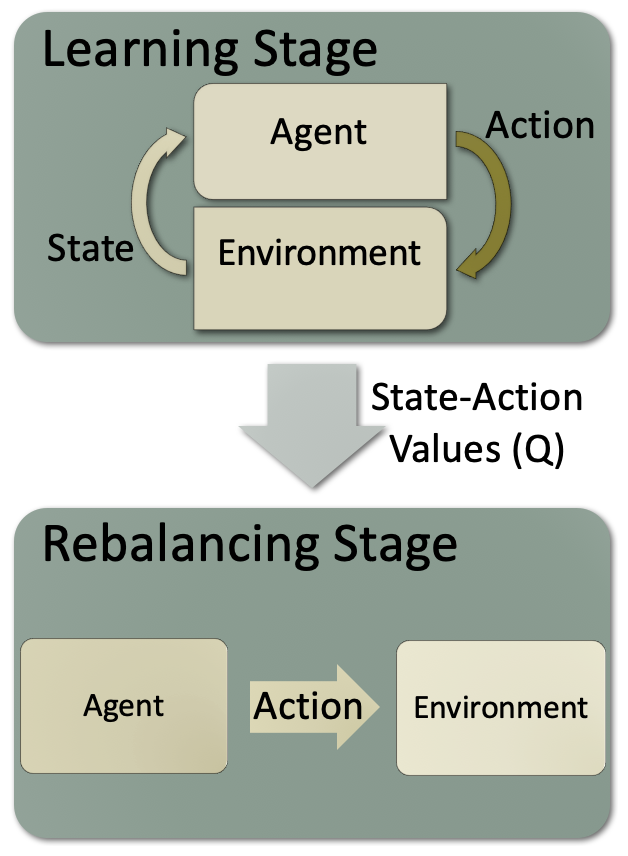
\includegraphics[scale=0.8]{procedure.png}
Fig. 1. Illustration of the proposed approach.


%%%%%%%%%%%%%%%%%%%%%%%%%%%%%%%%%%%%%%%%%%%%%%%%%%%%%%%%%%%%%%%%%%%%%%%%%%%%%%%%
\section{Problem formulation}
\subsection{Background Information}
Consider an environment discretized into a set of $\mathcal{N}$ stations (also can be viewed as discretized regions, as in [1]). Time is presented in discrete intervals of unit time $1$. The furthest time that will be considered is denoted as $T$.

Furthermore, let $M$ denote the total number of vehicles. Let $v^e_i$ denote the difference between the number of vehicles at or arriving at station $i$, and the number of passengers preparing to board an available vehicle at station $i$.[ TO DO: cite reactive paper]. Note that we assume that the vehicles arrive deterministically, or that no uncertainty is taken into account for travel times between two stations. 

%%%%%%%%%%%%%%%%%%%%%%%%%%%%%%%%%%%%%%%%%%%%%%%%%%%%%%%%%%
\subsection{MDP Model Description}
At every time step $t \in \{1,...,T-1,T\}$, a MDP, an \textit{agent} observes the environment and store the values of interest in the observation as its \textit{current state, $s_t$}. The agent then conducts an \textit{action $a_t$} following a certain policy, $\pi(s_t)$. At the end of this time step (or the beginning of time step $t+1$), a \textit{new state $s_{t+1}$} and a \textit{reward $r_t$} are observed. The definitions of MDP components are:\\

\noindent \textit{Agent}: Each vehicle is treated as an agent. Although this definition makes the problem a multiagent problem, it reduces the dimensions of actions, so that there is a smaller action space to explore. \\

\noindent \textit{State, $s_t$}: The state at time step $t$ is defined as a vector of length $2|N|$, concatenated with two $|N|$ dimensional vectors, $v^e$ and $o^m$. $v^e$ stores all elements of $v^e_i$. The vector $o^m$ is the one-hot vector with value 1 at where vehicle $m$'s current station is.[TO DO: DEFINE FINAL STATE DEFINITION] \\

\noindent \textit{Action, $a_t$}: An agent is only made to choose an action when it is idle. Consider an idle agent currently at station $i$. Its action is defined as $j$, where $j\in \mathcal{N}$. If $i = j$, then the agent remains idle at its current station. If $i \neq j$, the agent departs to go to station $j$. The dimension of the action space is therefore $\mathcal{N}$. \\

\noindent \textit{Reward, $r_t$}: The reward is equal to the average customer wait time at time $t$. [TO DO: DEFINE FINAL REWARD DEFINITION] \\ 

Lastly, from classical MDP definitions, we define the state-action value, $Q(s,a)$ as the expected utility if following an action $a$ from state $t$.

%%%%%%%%%%%%%%%%%%%%%%%%%%%%%%%%%%%%%%%%%%%%%
\subsection{Problem Formulation}
\subsubsection{Learning Stage}
The goal in the learning stage is to output accurate estimation of the state-action values, $Q(s,a)$ for any state-action pair $(s,a)$.

For state $s_t$ and action $a_t$ at time $t$, we define the predicted state-action values, $Q(s_t,a_t;\textbf{w})$ as the ${a_t}^{th}$ row of $\textbf{w}x_t$,
where $\textbf{w}$ is the weight matrix, and $x_t$ is the state vector $s_t$ plus a term accounting for bias. 

At each time step, we use new information in this time step to improve our prediction. The objective of the learning stage can therefore be formally written as:

\begin{equation}
    \min J(s_t,a_t;\textbf{w}) = [Q(s_t,a_t;\textbf{w}) - (r_t+\gamma  Q(s_{t+1},a_{t+1};\textbf{w}))]^2
\end{equation}
where $\gamma$ is the future reward discount factor, which is adjustable parameter.\\

%%%%%%%%%%%%%%%%%%%%%%%%%%%%%%%%%%%%%%%%%%%%%%%%%%%%%%%%%

\subsubsection{Rebalancing Stage}
Actions that give highest state-action values for each agent may be only optimal locally but not globally. At this stage, we aim to use the state-action values learned in the learning stage to find actions that maximize the sum of values of all cars. 

The objective of this stage is that for every time step $t$
\begin{equation}
        \min -\sum_m^M Q^m(s_t,a_t;\textbf{w})\forall i,j\in \mathcal{N}
\end{equation}
where $Q^m(s_t,a_t;\textbf{w})$ is the state-action value corresponding to vehicle $m$ taking action $a_t$ under state $s_t$. 

\section{Proposed Solution}
\subsection{Learning Stage}
Due to the large size of the state-space, we will use the SARSA with value-function approximation (VFA) algorithm to approximate the state-action values. Each vehicle at each time step is a data point that the algorithm use to update the weight matrix. To do this, vehicles' actions are performed sequentially. We create smaller simulated states, $\hat{s}_t$ that are updated every time a vehicle has been assigned an action. The algorithm is as follows:
\begin{algorithm}[H]
\caption{Learning Stage: SARSA with VFA}
\begin{algorithmic}
\For{each time step $t \in {0,1,...,T}$ }
    \State Observe $\hat{s}_t=s_t$
    \For{each vehicle $m$}
        \If {vehicle is idle}
            \State $a^m_t \leftarrow \pi(s_t)$ 
            \State $\hat{s}_t \leftarrow$ \textbf{simulate} $(a^m_t,s_t)$
        \EndIf
        \State Observe $r_{t-1}$
        \State $\textbf{w} \leftarrow \textbf{w} - \alpha \nabla_{ \textbf{w}} J(s_{t-1},a_{t-1};\textbf{w})$
    \EndFor
    \State\textbf{Assign} $\{a^1_t,a^2_t,...,a^M_t\}$
\EndFor
\end{algorithmic}
\end{algorithm}
 [TO DO: DEFINE PI. ADD derivation for derivative of J to appendix]
 
In this algorithm, we parameterize state-action values as a function of state, action and a weight matrix, in order to predict the values for unseen states as well. The algorithm approaches convergence as the objective in (1) is met.

By creating smaller simulated states and thereby making decisions sequentially, we can take into account of the actions of other agents while an agent performs action.  

\subsection{Rebalancing Stage}
In the rebalancing stage, we find the global optimum by assigning actions sequentially for each vehicle. The algorithm follows: 
\begin{algorithm}[H]
\caption{Rebalancing Stage: Performing Actions}
\begin{algorithmic}
\For{each time step $t \in {0,1,...,T}$}
    \State Observe $\hat{s}_t=s_t$
    \For{each vehicle $m$}
        \If {vehicle is idle}
            \State $a_t^m \leftarrow \argmax_a(Q(\hat{s}_t,a))$
            \State $\hat{s}_t \leftarrow$ \textbf{simulate}$(a^m_t,s_t)$
        \EndIf
    \EndFor
    \State\textbf{Assign}$\{a^1_t,a^2_t,...,a^M_t\}$
\EndFor
\end{algorithmic}
\end{algorithm}

\section{Simulation/Experiments}

\addtolength{\textheight}{-3cm}   % This command serves to balance the column lengths
                                  % on the last page of the document manually. It shortens
                                  % the textheight of the last page by a suitable amount.
                                  % This command does not take effect until the next page
                                  % so it should come on the page before the last. Make
                                  % sure that you do not shorten the textheight too much.

%%%%%%%%%%%%%%%%%%%%%%%%%%%%%%%%%%%%%%%%%%%%%%%%%%%%%%%%%%%%%%%%%%%%%%%%%%%%%%%%
%%%%%%%%%%%%%%%%%%%%%%%%%%%%%%%%%%%%%%%%%%%%%%%%%%%%%%%%%%%%%%%%%%%%%%%%%%%%%%%%
\section{Conclusions}

\subsection{Conclusions}

\bibliographystyle{unsrt} 
\bibliography{Biblio}  

\section*{Appendix --- style guidelines}

\subsection{Figures and Tables}

Position figures and tables at the tops and bottoms of columns.
Avoid placing them in the middle of columns. Large figures and tables
may span across both columns. Figure captions should be below the figures;
 table captions should be above the tables. Avoid placing figures and tables
  before their first mention in the text. Use the abbreviation ``Fig. 1'',
  even at the beginning of a sentence.
Figure axis labels are often a source of confusion.
Try to use words rather then symbols. As an example write the quantity ``Inductance",
 or ``Inductance L'', not just.
 Put units in parentheses. Do not label axes only with units.
 In the example, write ``Inductance (mH)'', or ``Inductance L (mH)'', not just ``mH''.
 Do not label axes with the ratio of quantities and units.
 For example, write ``Temperature (K)'', not ``Temperature/K''.

\subsection{Numbering}

Number reference citations consecutively in square brackets \cite{Garcia.ea:Auto89}.
 The sentence punctuation follows the brackets \cite{Garcia.ea:Auto89}.
 Refer simply to the reference number, as in \cite{Garcia.ea:Auto89}.
 Do not use ``ref. \cite{Garcia.ea:Auto89}'' or ``reference \cite{Garcia.ea:Auto89}''.
Number footnotes separately in superscripts\footnote{This is a footnote}
Place the actual footnote at the bottom of the column in which it is cited.
Do not put footnotes in the reference list.
Use letters for table footnotes (see Table I).

\subsection{Abbreviations and Acronyms}

Define abbreviations and acronyms the first time they are used in the text,
even after they have been defined in the abstract. Abbreviations such as
IEEE, SI, CGS, ac, dc, and rms do not have to be defined. Do not use
abbreviations in the title unless they are unavoidable.

\subsection{Equations}

Number equations consecutively with equation numbers in parentheses flush
 with the right margin, as in (1). To make your equations more compact
 you may use the solidus (/), the exp. function, or appropriate exponents.
  Italicize Roman symbols for quantities and variables, but not Greek symbols.
   Use a long dash rather then hyphen for a minus sign. Use parentheses to avoid
    ambiguities in the denominator.
Punctuate equations with commas or periods when they are part of a sentence:
$$\Gamma_2 a^2 + \Gamma_3 a^3 + \Gamma_4 a^4 + ... = \lambda \Lambda(x),$$
where $\lambda$ is an auxiliary parameter.

Be sure that the symbols in your equation have been defined before the
equation appears or immediately following.
Use ``(1),'' not ``Eq. (1)'' or ``Equation (1),''
except at the beginning of a sentence: ``Equation (1) is ...''.

%\begin{table}
%\caption{An Example of a Table}
%\label{table_example}
%\begin{center}
%\begin{tabular}{|c||c|}
%\hline
%One & Two\\
%\hline
%Three & Four\\
%\hline
%\end{tabular}
%\end{center}
%\end{table}

   \begin{figure}[thpb]
      \centering
      %\includegraphics[scale=1.0]{figurefile.jpg}
      \caption{Inductance of oscillation winding on amorphous
       magnetic core versus DC bias magnetic field}
      \label{figurelabel}
   \end{figure}




\end{document}
